\documentclass[../main.tex]{subfiles}

\begin{document}

\section{Networks}
In generale, un network \`e descritto da una matrice di adiacenza $\mathcal{A}_{ij}=\left\{0,1\right\}$ in cui la cella $(i,j)$ assume il valore $1$ se il nodo $i$ \`e connesso al nodo $j$, $0$ altrimenti.
Nei casi considerati in questo studio si assume sempre che $\mathcal{A}_{ij}=\mathcal{A}_{ji}$ (proprietà di simmetria).
Affiancata alla matrice di adiacenza si usa definire spesso la matrice dei pesi $\mathcal{W}_{ij}$, la quale definisce il peso di ciascun collegamento tra nodi.
In particolare, la matrice $\mathcal{W}_{ij}$ possiede le seguenti propiet\`a:
\begin{itemize}
    \item $\mathcal{A}_{ij} = 0 \Longrightarrow \mathcal{W}_{ij} = 0$;
    \item $\mathcal{A}_{ij} = 1 \Longrightarrow \mathcal{W}_{ij} \neq 0$.
\end{itemize}
Dalla matrice di adiacenza \`e possibile definire il grado del nodo $i$-esimo come
\begin{equation*}
    d_i=\sum_j\mathcal{A}_{ij}\\
\end{equation*}
che indica il numero dei link per ogni nodo.
\\Una volta note le matrici di adiacenza e il vettore dei gradi la matrice Laplaciana del network \`e definita come
\begin{equation}
    \mathcal{L}_{ij}=d_i\delta_{ij}-\mathcal{A}_{ij}
\end{equation}
ed ha le seguenti propriet\`a:
\begin{itemize}
    \item \`e semi-definita positiva;
    \item $\mathcal{L}_{ij}>0\Longleftrightarrow i=j$;
    \item $\sum_j\mathcal{L}_{ij}=\sum_i\mathcal{L}_{ij}=0$, quindi esiste un autovalore nullo $\lambda_0$ con corrispondente autovettore $\vec{v}_0=(1,\ldots,1)$;
    \item $\sum_i\mathcal{L}_{ii}=2m$, dove $m$ \`e il numero totale dei link.
\end{itemize}
\subsection{Random Walk su network}
Si assuma ora che la rete abbia in totale $M$ nodi e che ognuno di essi possa scambiare particelle coi suoi vicini.
Sia $\pi_{ij}$ la matrice stocastica che definisce la probabilità che una particella effettui il viaggio tra nodi $j\to i$.
Questa possiede le seguenti proprietà:
\begin{itemize}
    \item $\mathcal{A}_{ij}=0 \Longrightarrow \pi_{ij}=0$;
    \item $\sum_j\pi_{ij}=1$.
\end{itemize}
Assumendo inoltre di avere $N$ particelle nella rete, \`e possibile definire la funzione $\delta_\alpha(i,t)$ che vale $1$ se la particella $\alpha$ si trova nel nodo $i$ al tempo $t$, 0 altrimenti.
\\Ogni particella segue quindi la dinamica
\begin{equation*}
    \delta_\alpha(i,t+\Delta t)=\sum_j\xi_{ij}^\alpha\delta_\alpha(j,t)
\end{equation*}
dove $\xi_{ij}^\alpha$ \`e una matrice random che prende valori della base standard $\widehat{e}_i\in \mathbb{R}^M$ con probabilità $\pi_{ij}$.
Il numero di particelle nel nodo $i$ al tempo $t$ \`e dato da
\begin{equation*}
    n_i(t)=\sum_\alpha\delta_\alpha(i,t)
\end{equation*}
ed \`e possibile dimostrare \cite{RandomWalks} che la seguente equazione \`e un integrale del moto
\begin{equation}
    \sum_in_i(t)=N
\end{equation}

\section{Costruzione del modello}
Si consideri ora un network generato dalla matrice di adiacenza simmetrica $\mathcal{A}_{ij}$ i cui nodi rappresentano gli incroci di una rete stradale.
Alla matrice di adiacenza \`e associata una matrice dei pesi $\mathcal{S}_{ij} \geq 0$ che, associando un diverso peso ad ogni link, definisce la lunghezza delle strade.
Su questo network si definiscano ora le classi di agenti $C_{1},\ldots,C_{k}$, ognuna delle quali caratterizzata da un nodo sorgente $src$ e destinazione $dst$ e denotate come $C_{\alpha}(src,dst)$.
Ogni individuo dovr\`a, nel corso della simulazione, muovere tra i nodi $src\to dst$ in modo da seguire la geodetica, ossia il percorso pi\`u breve.
Il costo di un percorso, tuttavia, non viene calcolato sulla base della lunghezza: data la mobilit\`a dei veicoli, risulta pi\`u accurato considerando il tempo di percorrenza.
A tale fine si definisca ora un'altra matrice dei pesi $\mathcal{V}_{ij} \geq 0$ rappresentante la velocit\`a massima alla quale un agente pu\`o andare su una determinata strada.
L'elemento di matrice
\begin{equation}
    \mathcal{T}_{ij}=
    \begin{cases}
        \frac{\mathcal{S}_{ij}}{\mathcal{V}_{ij}} \quad& \mathcal{V}_{ij} \neq 0\\
        0 \quad& \mathcal{V}_{ij} = 0
    \end{cases}
\end{equation}
rappresenta dunque il costo temporale associato al link $i \to j$.\\
Discretizzando il tempo con un passo $\Delta t$, il costo di un percorso risulta esprimibile come
\begin{equation}
    G=c\Delta t
\end{equation}
dove $c \in \mathbb{N}$.
Nel limite di individui non interagenti tra di loro \`e quindi possibile calcolare costo della geodetica, chiamata \emph{best path}, come
\begin{equation}
    G_{\text{best}} = c_{\text{best}}\Delta t = \min \left\{\sum_{i=src}^{j=dst}\mathcal{T}_{ij}\right\}
    \label{eq:best_path}
\end{equation}
Si assuma ora che gli agenti muovano sulla rete seguendo un moto stile random walk.
Per ogni classe di individui $C_{\alpha}$ \`e quindi necessario definire una matrice stocastica (di transizione) $\pi_{ij}^{\alpha}$ con le propriet\`a descritte nella sezione precedente.
Nella realt\`a una strada ha una capacit\`a finita, intesa come numero massimo di veicoli presenti su di essa in un generico istante di tempo $t$.
Tale vincolo viene implementato nel modello tramite l'introduzione di una densit\`a massima $\rho_{max}$ posseduta da ogni strada.

\subsection{Algoritmo di evoluzione}
\`E ora necessario definire come i veicoli muovano effettivamente sul network.
La probabilit\`a di transizione di osgni classe $\pi_{ij}^{\alpha}$ viene assegnata nel modo seguente:
\begin{itemize}
    \item fissato il nodo di partenza $i$ si inizia a scorrere sul passo successivo nel nodo $j$;
    \item se il nodo $j$ si trova sul percorso $G_{\text{best}}$, definito dall'Eq. (\ref{eq:best_path}), allora viene assegnato un peso $\pi_{ij}=1$;
    \item altrimenti, se il link esiste ($\mathcal{A}_{ij} \neq 0$) viene assegnato un peso $\pi_{ij}=\tanh \beta T$, dove $\beta$ \`e un parametro di controllo del modello e $T$ rappresenta una temperatura statistica;
    \item una volta controllati tutti i possibili $j$ il vettore riga $i$-esimo viene poi normalizzato in modo tale da avere $\sum_j\pi_{ij}=1$.
\end{itemize}
Si osservi che grazie all'introduzione della temperatura statistica $T$, graficata in Fig. \ref{fig:temperature}, \`e possibile permettere agli agenti di ``sbagliare'' percorso e uscire dalla geodetica, introducendo cos\`i delle fluttuazioni.
Inoltre, per $T \to \infty$ l'evoluzione del sistema diventa equivalente ad un random walk su network in quanto ogni scelta di percorso ha la medesima probabilit\`a.
\begin{figure}[H]
    \centering
    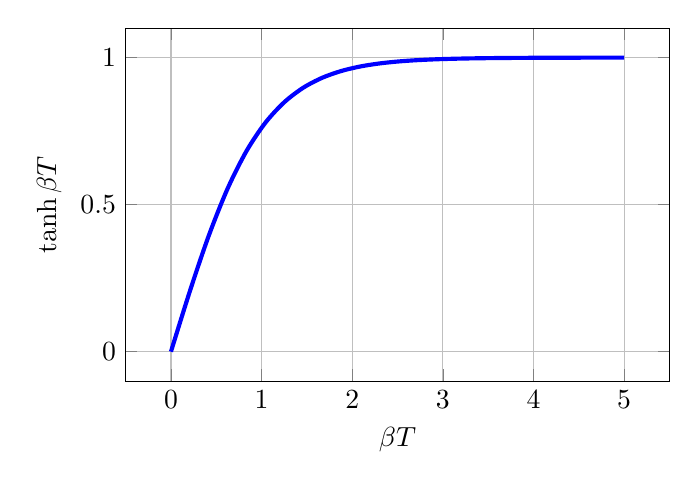
\begin{tikzpicture}
        \begin{axis}[
            grid = both,
            major grid style = {lightgray},
            minor grid style = {lightgray},
            width = 0.7\textwidth,
            height = 0.5\textwidth,
            xlabel = {$\beta T$},
            ylabel = {$\tanh \beta T$},]
            \addplot[
                domain = 0:5,
                smooth,
                color = blue,
                line width = 1.5pt,] {tanh(x)};
        \end{axis}
    \end{tikzpicture}
    \caption[Temperatura statistica]{\emph{Probabilit\`a di errore in funzione della temperatura statistica.}}
    \label{fig:temperature}
\end{figure}
Considerando ora un individuo generico appartente alla classe $C_{\alpha}$ si procede nel modo seguente:
\begin{itemize}
    \item si controlla se sia in grado di muoversi, quindi se $c = 0$. In caso negativo si sconta uno step temporale $c = c -1$ e si prosegue con gli altri veicoli;
    \item in caso affermativo, il passo successivo sarà deciso stocasticamente dalla matrice $\pi_{ij}^{\alpha}$;
    \item se la strada di arrivo \`e piena si perde uno step temporale, altrimenti l'individuo si immette sulla strada che connette i nodi $i \to j$ regolando la sua velocit\`a secondo la legge 
    \begin{equation}
        v(t) = v_{max}\left(1-k\frac{\rho(t)}{\rho_{max}}\right)
    \end{equation}
    dove $\rho(t)$ rappresenta la densit\`a di veicoli presenti sulla strada al tempo $t$ e $k$ \`e un parametro di controllo del modello;
    \item in base alla velocit\`a acquisita all'inviduo viene poi assegnata una nuova penalit\`a temporale $c = \frac{L}{v(t)\Delta t}$, con $L$ lunghezza della strada in cui si trova.
\end{itemize}
\begin{figure}[H]
    \centering
    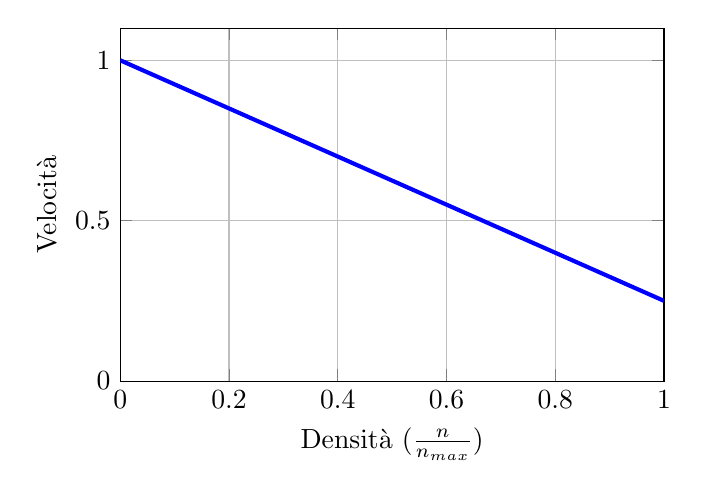
\begin{tikzpicture}
        \begin{axis}[
            grid = both,
            major grid style = {lightgray},
            minor grid style = {lightgray},
            ymin=0,
            xmin=0,
            xmax=1,
            width = 0.7\textwidth,
            height = 0.5\textwidth,
            xlabel = {Densità ($\frac{n}{n_{max}}$)},
            ylabel = {Velocità},]
        \addplot[
            domain = 0:1,
            smooth,
            color = blue,
            line width = 1.5pt,] {1-0.75*x};
        \end{axis}
    \end{tikzpicture}
    \caption[Velocità nel modello]{\emph{Ipotesi dell'andamento della velocità in funzione della densità per $k = 0.75$.}}
    \label{figure:velocity}
\end{figure}
Si noti come l'Eq. (\ref{eq:best_path}), graficata in Fig. \ref{figure:velocity}, tenda all'ipotesi di Greenshield per $k = 1$ (cfr. Eq. (\ref{figure:greenshield})). 


\end{document}